\documentclass[10pt]{article}

\usepackage[T1]{fontenc}
\usepackage[utf8]{inputenc}
\usepackage[brazilian]{babel}
\usepackage{hyphenat}
\usepackage{amsmath,amssymb,calrsfs,physics}
\usepackage[a4paper, margin=2cm]{geometry}
\usepackage{graphicx}
\graphicspath{ {./images/} }
\usepackage{textcomp}
\usepackage[export]{adjustbox}
\usepackage{multirow}
\usepackage{subcaption}
\usepackage{wrapfig}
\usepackage[colorlinks=true,linkcolor=blue]{hyperref}%
\usepackage{microtype} 			% para melhorias de justificação
\usepackage[ruled,vlined]{algorithm2e}
\usepackage{csquotes}
\usepackage{float}
\usepackage{tabularx}
\usepackage[backend=biber]{biblatex}
\addbibresource{refs.bib}

\begin{document}

% \maketitle

\begin{titlepage}
\begin{center}
{\large Universidade Federal de Minas Gerais\\
Escola de Engenharia \\
Curso de Graduação em Engenharia de Controle e Automação\\}

\vspace{6cm}
{\bf\Large Primeira Linha do Título\vspace{0.2cm}

Segunda Linha do Título, se Houver}
\vspace{4cm}

%\hspace{0.3\textwidth} \parbox{0.65\textwidth}
{\large André Sales Barbosa}
\vspace{2cm}  
   
\vspace{2cm}          
%\hspace{0.3\textwidth} 
{\large Orientador: Prof. Antônio de Pádua Braga, Dr.}\\


\vfill
%\hspace{0.3\textwidth} 
{\large Belo Horizonte, Dezembro de 2017 }
\end{center}

\end{titlepage}

\newpage
\clearpage
\thispagestyle{empty}


\begin{titlepage}

\centering
\textbf{Monografia}\\
\vspace{2cm}
\centering
\textbf{Título da Monografia}\\
\vspace{5cm} 

\parbox{1.0\textwidth} 
{\large 
Monografia submetida à banca examinadora
designada pelo Colegiado Didático do Curso de
Graduação em Engenharia de Controle e
Automação da Universidade Federal de Minas
Gerais, como parte dos requisitos para aprovação na
disciplina Projeto Final de Curso II.}

\vspace{7cm} 
\centering
Belo Horizonte, Dezembro de 2017

\end{titlepage}

\clearpage
\thispagestyle{empty}
\cleardoublepage

\tableofcontents

\section{Descrição do problema e solução proposta}

Esse trabalho de projeto de final de curso se dedica à implementação do algoritmo
 de reconhecimento de padrões para classificar movimentos.
Para isso faz-se o uso de uma placa de desenvolvimento do  microcontrolador ESP32 e um sensor 
acelerômetro MPU6050. O protótipo desenvolvido deverá reconhecer qual movimento foi aplicado
 ao objeto e exercer uma atuação a partir disso.
 A inspiração para o projeto veio do conceito de inteligência distribuída. Nessa abordagem o
 algoritmo de inteligência artificial é implementado nos dispositivos de borda ("edge"), evitando
 a transferência de dados para um processamento central.



% \begin{figure}[H]
%     \centering
%     \begin{subfigure}[b]{0.49\textwidth}
%         \centering
%         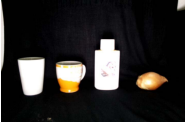
\includegraphics[scale=1.55]{images/input_image.png}
%         \caption{Foto sem tratamento}
%         \label{fig:celula_raw}
%     \end{subfigure}
%     \hfill
%     \begin{subfigure}[b]{0.49\textwidth}
%         \centering
%         %% substituir pela imagem correta depois
%         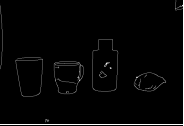
\includegraphics[scale=1.52]{images/output_image.png}
%         \caption{Após algoritmo de detecção de bordas}
%         \label{fig:detec_quinas}
%     \end{subfigure}
%     \caption{Fotos antes e depois do algoritmo de detecção de bordas}
%     \label{fig:celulas}
% \end{figure}

% \section{Resultados}

% Todas as operações de processamento de imagens realizadas na pesquisa utilizaram os módulos de \cite{opencv}. Utilizando a rotina para detecção de bordas, mesmo com a configuração da captura da foto não sendo ideal, a aplicação de operações morfológicas \ref{eq:dilation}\ref{eq:erosion} na imagem toda, é possível atingir níveis de acurácia elevados, como indicado na tabela abaixo.

% \begin{equation}
%     dst(x,y)=max_{(x',y'):element(x',y')!=0}src(x+x',y+y')
%     \label{eq:dilation}
% \end{equation}

% \begin{equation}
%     dst(x,y)=min_{(x',y'):element(x',y')!=0}src(x+x',y+y')
%     \label{eq:erosion}
% \end{equation}

\listoffigures
\printbibliography
\end{document}
